\documentclass[11pt,a4paper]{article}
 
\usepackage{polski}
\usepackage[utf8]{inputenc} %utf-8 żeby nie było problemów z przenoszeniem między windowsem a linuxem
\usepackage{graphicx}
\usepackage{listings}
\usepackage{indentfirst}

%lokalne makro na komendę
\newcommand{\HRule}{\rule{\linewidth}{0.5mm}}

\setlength\parindent{24pt}
\oddsidemargin=20pt
\textwidth=420pt



 
\begin{document}

%strona tytułowa
\begin{titlepage}
\begin{center}
%nagłówek uczelni
\textsc{\LARGE Politechnika Warszawska}\\[0.5cm]
\textsc{\Large Wydział Elektroniki i Technik Informacyjnych}\\
\textsc{\Large Instytut Automatyki i Informatyki Stosowanej}\\[1.5cm]

\textsc{\Large Sprawozdanie z pracowni dyplomowej inżynierskiej I} \\[0.5cm]
%tytuł między kreskami
\HRule \\[0.4cm]
{ \huge \bfseries Generator raportów z baz danych w technologii XSL-FO  bazujący na wzorcach \\[0.4cm]}
\HRule \\[1.5cm]

%autor
\begin{minipage} {0.4\textwidth}
\begin{flushleft} \large
\emph{Autor:}\\
 Maciej Kucharski 
\end{flushleft}
\end{minipage}
%promotor
\begin{minipage} {0.4\textwidth}
\begin{flushright} \large

\emph{Opiekun:}\\
doc. dr inż. Tomasz Traczyk

\end{flushright}
\end{minipage}	
\vfill
\large Semestr 13Z

	\end{center}
\end{titlepage}
 
\tableofcontents
\newpage

%Cel pracy
\section{Cel pracy} \label{sec:cel}
XSL-FO to zaawansowana, ale mało popularna technologia, umożliwiająca m.in. tworzenie publikacji na wysokim poziomie poligraficznym. Za pomocą tej technologii można tworzyć również zaawansowane i atrakcyjne graficznie raporty z bazy danych. W szczególności narzędzie Oracle Application Express potrafi współpracować z dość popularnym procesorem XSL-FO Apache FOP. Dane pobrane z bazy należy odpowiednio przekształcić np. za pomocą XSLT do postaci XSL-FO.

Celem pracy jest opracowanie i stworzenie narzędzia, które potrafiłoby na podstawie specyfikacji danych źródłowych oraz wzorca wyglądu raportu wygenerować odpowiednie skrypty XSLT, przekształcające dane w dokumenty XSL-FO, dające po przetworzeniu wynikowe raporty. Narzędzie ma działać podobnie do Oracle XML (BI) Publishera, jednak w znacznie węższym zakresie i z prostszymi wzorcami.

W następnych rozdziałach zaprezentowane zostaną narzędzia i technologie wykorzystane w niniejszej pracy.

%najpierw XML ogólnie
\section{XML} \label{sec:xml}
XML (Extensible Markup Language) to standard organizacji W3C służący do liniowego przedstawiania danych semistrukturalnych. Język XML jest podobny do popularnego HTML-a. Głównym przeznaczeniem XML-a jest elastyczna reprezentacja danych, które są reprezentowane za pomocą tzw.znaczników. Znacznikiem są zarówno elementy, jak i atrybuty. Elementy składają się z otwierającego znacznika, zamykającego znacznika i wszystkich informacji między nimi. Może to być zarówno tekst, jak i zagnieżdżone na dowolną głębokość podelementy. 

Atrybuty służą przekazaniu dodatkowych informacji o elementach i obejmują pary klucz-wartość. Poniższy listing prezentuje przykładowe dane w zapisie spełniającym minimalne wymogi XML:\\

\lstset{language=XML}
\begin{lstlisting}[frame=single,caption=Prosty XML,label=simplexml]
<?xml version="1.0" encoding="utf-8" standalone="yes" ?>
<root>
	<element1>wartosc</element1>
	<element2 atrybut="wartosc_atrybutu">wartosc</element2>
	<element3 atrybut="wartosc" />
</root>
\end{lstlisting}

Element \textless root\textgreater \ jest głównym elementem dokumentu XML, tzw. root element. Element takiego typu musi występować w każdym XML-u.

Dzięki zdefiniowaniu DTD bądź XMLSchema możliwe jest określenie, jakie elementy i atrybuty występują w dokumencie.Wtedy wartość atrybutu standalone wynosi "false".  Parser wczytujący dokument może dzięki temu walidować jego poprawność. W praktyce DTD jest żadko stosowane ze względu na fakt, że jest oddzielnym językiem. Z kolei XMLSchema jest określana za pomocą XML.

%teraz XSLT
\section{XSLT} \label{sec:xslt}
Język XSLT (Extensible Stylesheet Language for Transformations) to standard opracowany przez W3C. Może być wykorzystany do przekształcania do przekształcenia dokumentu z jednej postaci na inną lub podobnie, jak XPath lub XQuery, do pobierania danych z dokumentów. Specyfikacja w XSLT jest dokumentem XML zwanym arkuszem stylów. Znaczniki stosowane w XSLT pochodzą z określonej przestrzeni nazw. Poniższy listing prezentuje ogólny arkusz stylów:\\

\lstset{language=XSLT}
\begin{lstlisting}[frame=single,caption=Ogólny arkusz XSLT,label=simplexslt]
<?xml version="1.0" encoding="utf-8" ?>
<xsl:stylesheet 
	xmlns:xsl="http://www.w3.org/1999/XSL/Transform">
	...
</xsl:stylesheet>
\end{lstlisting}

W jednym arkuszu stylów może być zdefiniowanych wiele szablonów. Stosowanie arkusza stylów do dokumentu XML polega na przeglądaniu listy szablonów zdefiniowanych w arkuszu do momentu znalezienia tego, który pasuje do elementu korzenia. Dla elementów zagnieżdżonych należy ponownie przeszukać listę szablonów. Poniższy listing prezentuje strukturę szablonu XSLT:\\
\lstset{language=XSLT}
\begin{lstlisting}[frame=single,caption=Ogólny szablon XSLT,label=simplexsltszablon]
<xsl:template match="wyrazenie XPath">
	...wynik transformacji...
</xsl:template>
\end{lstlisting}

Arkusz XSLT pozwala również na stosowanie pętli i instrukcji warunkowych.


%wreszcie XSL-FO
\section{XSL-FO} \label{sec:xslfo}
XSL Formatting Objects to język oparty na XML, stosowany do formatowania dokumentów. Główną ideą postania tej specyfikacji jest fakt, że w przeciwnieństwie do HTML, czy XHTML, dokumenty XML nie zawierają wbudowanego układu wizualnego. XSL-FO jest językiem, który może zostać użyty do nadania dokumentowi XML układu na stronie, kolorów, czcionek itd. z przeznaczeniem wyniku dla różnych mediów, np. ekranu lub drukarki. W tym sensie pełni funkcję podobną do stylów CSS, jednak jest bardziej elastyczny i daje większe możliwości, zwłaszcza jeśli chodzi np. o stronicowanie i przewijanie.

% ogólna problematyka raportów
\section{Problematyka raportów}\label{sec:raport}
Raport to standardowa forma dokumentu biznesowego, który prezentuje informacje jakościowe i ilościowe w logiczny sposób. Raporty takie należą do najważniejszych dokumentów przedsiębiorstwa. Raport przedstawia widok informacji odpowiedni dla danej grupy odbiorców. Jego funkcje to np.
ocena wydajności biznesowej, umożliwiająca szybkie sprawdzenie stanu oraz monitorowanie stopnia realizacji strategicznych celów przedsiębiorstwa, podsumowywanie kluczowych wskaźników biznesu, czy prezentacja miar biznesowych w oparciu o różne statystyki. W następnych punktach zostaną przedstawione najczęściej wykorzystywane wzorce raportów.
%master-detail
\subsection{Raport typu \emph{master-detail}}\label{sec:master_detail}
Ten typ raportu prezentuje wartości pełniące funkcję nadrzędnych względem innych oraz szczegóły aktualnie wybranej pozycji. W zasadzie odpowiada strukturze typowego dokumentu, np. faktury. Ten typ raportu może być zastosowany przy związkach typu jeden-wiele. Zarówno obszar nadrzędny jak i podrzędny może być listą lub drzewem pozycji, co umożliwia wprowadzanie wielu stopni podrzędności, przy czym obszar podrzędny zwykle jest umieszczony pod lub obok obszaru nadrzędnego. Przykładem może być spis pozycji wchodzących w skład danego zamówienia lub działy przedsiębiorstwa wraz ze spisem pracowników każdego z nich.
%break groups
\subsection{Raporty z grupami łamiącymi (\emph{break groups})}\label{sec:break_groups}
Ten typ raportu polega na podziale wierszy trafiających do raportu na grupy o jednakowych wartościach w wyróżnionych kolumnach. Każdą z takich grup można odpowiednio obsłużyć, np. opatrywać je nagłówkami, czy wyliczać dla nich podsumowania. Taka struktura umożliwia dosyć elastyczną prezentację tych samych danych. Załóżmy, że mamy bazę pracowników zatrudnionych w różnych działach. Mogą oni być pogrupowani na podstawie działów, w których są zatrudnieni, następnie, w obrębie działów, można podzielić ich np. ze względu na lata pracy, a dodatkowo np. ze względu na przedziały ich zarobków. 
%macierzowy
\subsection{Raport macierzowy (krzyżowy)}\label{sec:macierzowy}
Raport macierzowy prezentuje związki między dwoma wymiarami. Takie raporty są często wykorzystywane przy różnego rodzaju ankietach. Prezentują związki między dwoma zmiennymi i ułatwiają znalezienie między nimi zależności. Struktura tego raportu przypomina arkusz kalkulacyjny programu Exel. Ułatwia to wspólne prezentacje danych, które pozornie nie mają ze sobą związku. Przykładem może być analiza ankiety, z której wynika na przykład, że pewien model samochodu sprzedaje się lepiej w pewnych województwach.


% opis Apache FOP
\section{Apache FOP}\label{sec:fop}
Apache FOP (\emph{Formatting Objects Processor}) jest programem napisanym w języku \emph{Java}, który konwertuje pliki zapisane w formacie XSL-FO na pliki w formacie PDF lub innych drukowalnych, m.in. RTF czy PostScript. Najnowsza stabilna wersja jest w znacznym stopniu zgodna ze specyfikacją XSL-FO 1.1. 

FOP może być wykorzystywane zarówno jako niezależna aplikacja uruchamiana np. z wiersza poleceń, jak i biblioteka Javy, dzięki czemu może być wykorzystany w każdej aplikacji tworzonej w języku Java. FOP umożliwia również przetwarzanie danych w formacie XML przy użyciu odpowiednich transformacji XSLT.

%raporty z apexa
\section{Raportowanie w ApEx}\label{sec:raporapex}
Oracle Application Express sam w sobie nie generuje raportów w formacie PDF. Aby to umożliwić, należy wykorzystać zewnętrzne narzędzie: Oracle XML (BI) Publishera lub Apache FOP uruchamianego jako serwlet na serwerze aplikacyjnym. W tej pracy zastosowana będzie tylko ostatnia metoda.

Schemat poglądowy wykorzystania FOP przez ApExa prezentuje obrazek \ref{fop:apex_usage}:\\

\begin{figure}[h]
\centering
\caption{Sposób wykorzystania FOP przez ApExa}
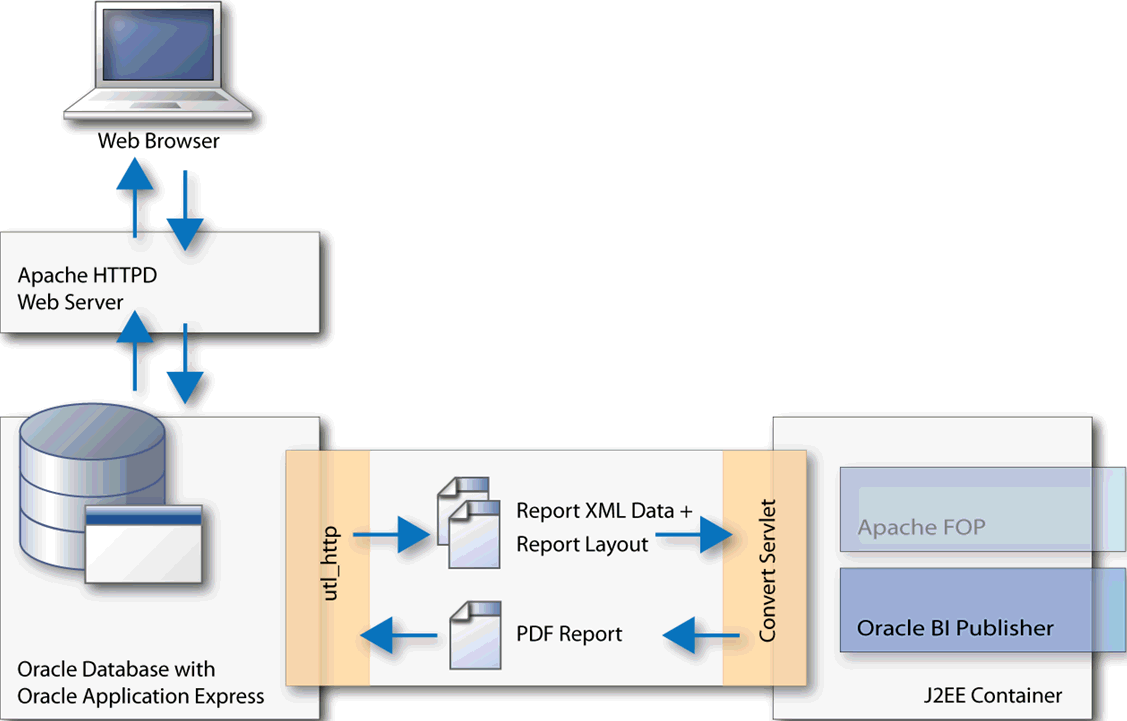
\includegraphics[scale=0.5]{apex_fop_usage}
\label{fop:apex_usage}
\end{figure}


Wersja 4.2.2 Application Express pozwala na stosowanie własnych wzorców wyglądu raportu zapisanych w XSL-FO. Istnieją darmowe narzędzia za pomocą których można wczytać dane w formacie XML, dostosować np. ich rozmieszczenie na stronie raportu metodą \emph{drag\&drop}, a następnie wygenerować skrypt XSLT transformujący dane na wynikową stronę raportu. 

%Format wzorca wyglądu
\section{Format zapisu wzorca wyglądu raportu}\label{sec:formatywzorce}
Aby możliwe było wygenerowanie raportu, niezbędny jest wzorzec jego wyglądu. Należy wybrać jakiś format spośród wielu istniejących, przy czym głównym czynnikiem jest łatwość przetwarzania i istnienie darmowych narzędzi do graficznej edycji. W związku z tym najsensowniejszym rozwiązaniem wydają się formaty bazujące na XML: SVG lub XSL-FO, a to ze względu na istnienie wielu parserów XML w praktycznie dowolnych językach programowania. Dla obu standardów istnieją narzędzia wspomniane wcześniej; dla SVG jest to np. open source'owy \emph{SVG-edit} działający w przeglądarce, bądź bardziej zaawansowany \emph{InkScape}. Dla XSL-FO niestety trudniej znaleźć darmowe oprogramowanie, po dłuższych poszukiwaniach okazało się, że darmowe wersje testowe programów takich, jak np. \emph{XF Designer}, czy \emph{J4LFOP} niefortunnie mają zablokowaną opcję eksportu XSL-FO. 

Ostatecznie jako wzorzec zostanie wykorzystany format SVG ze względu na dostępność narzędzi określanych jako WYSIWYG (\emph{What You See Is What You Get}).

%jak widzę tę apkę?
\section{Koncepcja realizacji aplikacji}
W tym rozdziale zostanie przedstawione zastosowanie przygotowywanego narzędzia, określone zostaną dane wejściowe, przybliżony sposób ich przetwarzania oraz określony zostanie wynik działania aplikacji.

\subsection{Zastosowanie}\label{sec:appZast}
W celu zapewnienia jednakowego wyglądu raportu niezależnie od platformy najlepiej jest zapisywać raport w formacie PDF. Żeby to zrobić, ApEx potrzebuje danych wejściowych w XML oraz arkusza XSLT, co skutkuje wygenerowaniem pliku w formacie XSL-FO. Ten z kolei jest wysyłany do FOP, co skutuje powstaniem pliku PDF. Przygotowywane narzędzie ma właśnie na celu przygotowanie arkusza XSLT dla potrzeb ApExa. Drugą możliwością jest również bezpośrednie skorzystanie z wygenerowanego pliku XSLT i uruchomienie FOP z poziomu wiersza poleceń przez aplikację. 

\subsection{Dane wejściowe}\label{sec:appDane}
Dla uproszczenia konstrukcji aplikacji zakłada się, że dane do raportu zostaną dostarczone w pliku XML, przy czym jego struktura jest odpowiednio określona. Ogólny schemat danych XML generowanych przez ApExa jest przedstawiony na listingu \ref{rap:apex}.\\

\lstset{language=XML}
\begin{lstlisting}[frame=single,caption=Ogólna postać dokumentu XML z danymi pochodzącymi z ApExa,label=rap:apex]
<?xml version="1.0" encoding="UTF-8"?>
<DOCUMENT>
 <ROWSET>
  <ROW>
    <KOLUMNA1>...</KOLUMNA1>
    <KOLUMNA2>...</KOLUMNA2>
       ...	
  </ROW>
  <ROW>....</ROW>
 </ROWSET>
</DOCUMENT>
\end{lstlisting}

W dokumencie mogą być również zawarte dowolne dodatkowe informacje takie, jak np. nazwa użytkownika generującego raport, datę, nazwę aplikacji w ApExie lub wartość znajdująca się w określonym regionie strony w ApExie. Fakt ten jest wykorzystywany do przekazania danych pozycji nadrzędnej przy raporcie \emph{master-detail}. Przykładowy dokument XML z danymi dla raportu \emph{master-detail} przedstawia listing \ref{strukturaDanychMD}. Wpis \emph{P8\_DEPTNO} oznacza kolumnę o nazwie \emph{DEPTNO} znajdującą się na stronie o numerze 8 w aplikacji stworzonej poprzez ApExa.


\lstset{language=XML}
\begin{lstlisting}[frame=single,caption=Struktura pliku z danymi wejściowymi dla raportu master-detail,label=strukturaDanychMD]
<?xml version="1.0" encoding="UTF-8"?>
<DOCUMENT>
    <P8_DEPTNO></P8_DEPTNO>
    <P8_DNAME></P8_DNAME>
    <P8_LOC></P8_LOC>
    <REGION ID="0">
        <ROWSET>
            <ROW>
                <EMPNO></EMPNO>
                <ENAME></ENAME>
                <JOB></JOB>
                <MGR></MGR>
                <HIREDATE></HIREDATE>
                <SAL></SAL>
                <COMM></COMM>
                <DEPTNO></DEPTNO>
            </ROW>
        </ROWSET>
    </REGION>
</DOCUMENT>
\end{lstlisting}


Dla raportów z grupami łamiącymi zakładana struktura właściwie odpowiada strukturze ogólnego dokumentu, przy czym dodatkowo jest wymagane, żeby zapytanie SQL pobierające dane do raportu posiadało klauzulę \emph{ORDER BY} sortującą dane według odpowiednich kolumn.

Struktura danych dla raportu macierzowego będzie podobna do tej dla raportu \emph{master-detail}. Różnicą będzie nie występowanie wartości z regionu strony jako danej dodatkowej oraz występowanie dodatkowej kolumny dla każdego wiersza. Przykładowy plik jest zaprezentowana na listingu \ref{strukturaDanychMAtrix}. Fragment ten prezentuje średnie zarobki na określonym stanowisku w działach o podanych numerach identyfikacyjnych.

\lstset{language=XML}
\begin{lstlisting}[frame=single,caption=Zakładana struktura pliku z danymi wejściowymi dla raportu macierzowego,label=strukturaDanychMAtrix]
<?xml version="1.0" encoding="UTF-8"?>
<DOCUMENT>
    <REGION ID="0">
        <ROWSET>
            <ROW>
                <JOB>CLERK</JOB>
                <10>1300</10>
                <20>950</20>
                <30>950</30>
                <40></40>
            </ROW>
        </ROWSET>
    </REGION>
</DOCUMENT>
\end{lstlisting}


Dodatkową daną wejściową będzie wzorzec wyglądu raportu. Będzie on zapisany w formacie SVG, jak zostało to zaznaczone w rozdziale \ref{sec:formatywzorce}.

\subsection{Sposób przetwarzania danych}\label{sec:appPrzetwarzanie}
Na początku działania do pliku wyjściowego dodawane są elementy stałe, tj. nagłówek samego XML oraz określenie właściwej przestrzeni nazw. Następnie rozpoczyna się przetwarzanie samego wzorca. Wiele elementów występujących we wzorcu stworzonym w programie \emph{InkScape} jest zbędnych dla potrzeb tworzenia raportu, dlatego w celu oszczędności pamięci warto rozważyć wstępne filtrowanie zawartości pliku przed jego wczytaniem. Następnie, analizując położenie wszystkich elementów wzorca można określić ogólne parametry strony raportu takie jak np. marginesy, rozmiar strony czy wymiary komórek tabeli. W dalszym przetwarzaniu biorą udział również dane. Dalsze postępowanie będzie zależne od typu raportu wybranego przez użytkownika. W przypadku raportu \emph{master-detail} wystąpienie elementu nadrzędnego oznacza powstanie nowego bloku (w sensie zgodnym z terminologią XSL-FO) zawierającego wartości elementu oraz (w przypadku niepustego zbioru elementów podrzędnych) kolejnego bloku składającego się z tabeli zawierającej pozycje podrzędne zrealizowaną za pomocą konstrukcji \emph{fo:table}. Warto byłoby skonstruować schemat przetwarzania tak, aby umożliwiał zastosowanie wielu stopni podrzędności. Fakt, że element jest nadrzędny w stosunku do innego może być wykrywany poprzez sprawdzenie, czy pierwszy z jego elementów-dzieci ma własnych potomków. W dość ogólnym rysie wyglądałoby to jak na poniższym listingu (zakładając strukturę taką jak na listingu z rodziału \ref{sec:appDane}:\\

\lstset{language=XML}
\begin{lstlisting}[frame=single,caption=Przykładowa struktura pliku XSL-FO,label=strukturaXSL]
<fo:block>
   kolumna1 kolumna2....
   wartosc1 wartosc2...
   <fo:block>
     kolumna1 kolumna2....
     wartosc1 wartosc2...	
  </fo:block>
</fo:block>


\end{lstlisting}

Dla raportu z wykorzystaniem grup łamiących podejście będzie podobne z tym, że wystąpienie zgodnej wartości atrybutu względem którego ma nastąpić grupowanie spowoduje wstawienie pustego bloku jako wartość komórki w wierszu tabeli.

Odwzorowanie raportu macierzowego będzie wymagało innego podejścia do przetwarzania danych, niż w poprzednim przypadku. Ze względu na strukturę tego typu raportu, należy przetwarzać daną kolumnę jednocześnie dla wszystkich wierszy wchodzących w skład raportu. Ponadto pierwsza kolumna wchodząca w skład każdego wiersza będzie zawierać nie konkretną wartość, a odpowiednią nazwę.

Oczywiście ostatecznie do wyjściowego arkusza XSLT musi zostać dopisana transformacja tworząca odpowiednie struktury XSL-FO. Ponieważ zapisanie transformacji XSLT wymaga podania wyrażenia XPath odpowiadającego transformowanym znacznikom, podczas przetwarzania musi być pamiętana przebyta ścieżka.

\subsection{Dane wyjściowe}\label{sec:appOutput}
 Efektem działania aplikacji ma być plik z arkuszem transformacji XSLT. Będzie on mógł zostać wykorzystany przez ApExa do wygenerowania pliku dokumentu w formacie XSL-FO, co umożliwi generację pliku PDF przy użyciu FOP.

\subsection{Wykorzystane technologie} \label{sec:appTech}
Ze względu na łatwość przetwarzania dokumentów XML wykorzystanych zostanie wykorzystujący maszynę wirtualną \emph{Javy} język \emph{Groovy}. Nawiązując do działania FOP, dobrym pomysłem mogłoby okazać się również przygotowanie narzędzia do działania na serwerze aplikacyjnym. Mogłoby to ułatwić tworzenie infrastruktury służącej do raportowania. Ponadto ApEx umożliwia wywołanie zewnętrznych usług, dzięki czemu proces zostałby usprawniony poprzez ograniczenie konieczności ingerencji człowieka. W takim przypadku wygodnie będzie skorzystać z istniejących bibliotek i frameworków do tworzenia aplikacji webowych. Dodatkowo do zarządzania dodatkowymi zależnościami i usprawienia procesu budowania wykorzystane zostanie narzędzie \emph{Apache Maven}.

\section{Dalsze plany}\label{sec:plany}
W następnych etapach przygotowania pracy planowane jest przede wszystkim uszczegółowienie opisu przetwarzania danych w taki sposób, aby dało się na jego podstawie rozpocząć implementację aplikacji realizującej funkcjonalność będącą celem pracy. 
\end{document}

